\documentclass[11pt,xcolor={dvipsnames},hyperref={pdftex,pdfpagemode=UseNone,hidelinks,pdfdisplaydoctitle=true},usepdftitle=false]{beamer}
\usepackage{presentation}[aspectratio=169]
\usepackage{math}
\usepackage{mathtools}
\usepackage{mleftright}

% Enter title of presentation PDF:
\hypersetup{pdftitle={Aggregate Shocks, Taxes, and Debt Management I}}
% Enter link to PDF file with figures:
\newcommand{\pdf}{figures.pdf}

\begin{document}
% Enter presentation title:
\title{Aggregate Shocks, Taxes, and Debt Management I}
\subtitle{Fiscal and Monetary Policy 2023}
% Enter presentation information:

% Enter presentation authors:
\author{Piotr Żoch}%
% Enter presentation location and date (optional; comment line if not needed):
\frame{\titlepage}

% Fill out content of presentation:
\begin{frame}{Plan}
    \begin{itemize}
    \item How \al{should} the government change taxes and debt in response
    to changes in purchases?
    \item For example: \al{should} it finance war spending in the same way
    as public education?
    \item This is a \al{normative} question, but to the extent real world
    governments behave according to prescriptions of models we will see
    in class, it will also be a \al{positive theory} of government debt
    and taxes.
    \end{itemize}
\end{frame}


\begin{frame}{Plan}

    \begin{itemize}
    \item We will study optimal taxation and debt policy in two environments:
    \begin{itemize}
    \item \alb{incomplete markets}: the government can buy or sell only a limited
    set of securities, often only a single risk-free security.
    \item \alr{complete markets}: the government can buy or sell claims contingent
    on all possible states of the world.
    \end{itemize}
    \item We will first study some reduced form models and then proceed to optimal
    taxation in a competitive equilibrium (Lucas and Stokey, 1983).
    \end{itemize}
\end{frame}
    %
    \begin{frame}
        \heading{Reduced form models}
    \end{frame}

    \begin{frame}{Incomplete Markets}
    \begin{itemize}
    \item We study the following problem based on Barro (1979):
    \begin{itemize}
    \item the government uses taxes $\tau_{t}$ to finance \emph{stochastic}
    purchases $g_{t}$;
    \item  $D\left(\tau_{t}\right)$  is the deadweight loss of taxes;
    \item the government wants to finance $g_{t}$ in a way that minimizes the
    expected value of present discounted deadweight loss of taxes: 
    \[
    \min[\bc{\tau_t}_{t=0}^\infty] \E[0] \sum_{t=0}^\infty \bs{\bp{\frac{1}{1+r}}^t D\bp{\tau_t}}
    \]
    where $1/\left(1+r\right)$ is the (gross) rate at which the government
    discounts the future.
    \end{itemize}
    \end{itemize}
    \end{frame}
    %
    \begin{frame}{Incomplete Markets}
    \begin{itemize}
    \item Assume that $g_{t}$ is governed by an $N$ state Markov chain.
    \item The state of the world is given by $s_{t}$ that follows a Markov
    chain with a transition probability matrix $P$: 
    \begin{align*}
    P_{ij} & =P\bc{s_{t+1}=\bar{s}_{j}\mid s_{t}=\bar{s}_{i}}. 
    \end{align*}
    \item Government spending $\bc{g_t}$ obeys 
    \begin{align*}
    g_{t} & =\begin{cases}
    g_{1} & \text{if}\;s_{t}=\bar{s}_{1}\\
    \vdots\\
    g_{N} & \text{if}\;s_{t}=\bar{s}_{N}.
    \end{cases}
    \end{align*}
    \end{itemize}
    \end{frame}
    %
    
    
    \begin{frame}{Incomplete Markets}
    \begin{itemize}
    \item The government can issue only \alg{one period, non-state contingent} debt (\alb{incomplete markets}) at price $1/\left(1+r\right)$,
    equal to the discount rate. 
    \item Government problem:
    \begin{align*}
     &  \min[\bc{\tau_t}_{t=0}^\infty] \E[0] \sum_{t=0}^\infty \bs{\bp{\frac{1}{1+r}}^t D\bp{\tau_t}}\\
    \text{s.t.}\quad & g_{t}+b_{t}=\frac{1}{1+r}b_{t+1}+\tau_{t}
    \end{align*}
    and, in addition, we assume 
    \[
        \E[0] \bs{\bp{\frac{1}{1+r}}^t b^2_t} \le \infty
    \]
    \end{itemize}
    \end{frame}
    %
    \begin{frame}{Digression on Bellman equations}
    \begin{itemize}
    \item How to solve the above problem? 
    \item My recommendation is to write it in a \emph{recursive} form: 
    \begin{align*}
    V\bp{b,g} & =\min[\tau] D\bp{\tau}+\frac{1}{1+r}\E\bs{V\bp{b',g'} \mid g }\\
    \text{s.t.}\quad & g+b=\frac{1}{1+r}b'+\tau
    \end{align*}
    where $x$ denotes current variables $\bp{x_{t}}$ and $x'$ denotes
    variables in the next period $\bp{x_{t+1}}$. 
    \item It looks like a two period problem (instead of infinite horizon)
    -- the ``only'' issue is that we do not know $V\bp{b,g}$
    (and it appears on the right hand side). 
    \item More on that in, for example, my Quantitative Economics course. 
    \end{itemize}
    \end{frame}
    %
    \begin{frame}{Digression on Bellman equations}
    \begin{itemize}
    \item Write
    \begin{align*}
        V\bp{b,g} & =\min[\tau] D\bp{\tau}+\frac{1}{1+r}\E\bs{V\bp{\bp{1+r}\bp{g+b-\tau},g'} \mid g }
    \end{align*}
    and differentiate with respect to $\tau$ to get the \alg{first order condition}:
    \[
    D'\bp{\tau}=\E\bs{\pd{V\bp{b',g'}}{b'} \mathrel{\Big|} g}   \]
    \item How to get $V'\bp{b',g'}\coloneqq \pdx{V\bp{b',g'}}{b'}?$
    \end{itemize}
    \end{frame}
    %
    \begin{frame}{Digression on Bellman equations}
    \begin{itemize}
    \item Write
    \begin{align*}
    V\bp{b,g} & = D\bp{g+b-\frac{1}{1+r}b'}+\frac{1}{1+r}\E\bs{V\bp{b',g'}\mid g}
    \end{align*}
    (note: there is no $\min_{\tau}$) and differentiate with respect to $b$: 
    \begin{align*}
    V'\bp{b,g} & =D'\bp{\tau}.
    \end{align*}
    This is the \alg{ envelope condition} and it implies
    \begin{align*}
    V'\bp{b',g'} & =D'\bp{\tau'}.
    \end{align*}
    \item \al{Important:} do not write $b'=b'\bp{b,g}$ or anything like
    that, these terms drop out anyway (why?).
    \end{itemize}
    \end{frame}
    %
    \begin{frame}{Digression on Bellman equations}
    \begin{itemize}
    \item The \alg{first order condition} 
    \[
        D'\bp{\tau}=\E\bs{\pd{V\bp{b',g'}}{b'} \mathrel{\Big|} g}  
    \]
    together with the \alg{envelope condition}
    \begin{align*}
        V'\bp{b',g'}  =D'\bp{\tau'}
    \end{align*}
    give us the \alg{Euler equation} 
    \begin{align*}
        D'\bp{\tau_t}  =\E[t]\bs{D'\bp{\tau_{t+1}}}
    \end{align*}
    \end{itemize}
    \end{frame}
    %
    \begin{frame}{Incomplete Markets}
    
    \begin{itemize}
    \item Solution to the government's problem is characterized by the first
    order condition 
    \[ D'\bp{\tau} =\E[t]\bs{D'\bp{\tau'}} .\]       
    \vspace{-0.76cm} 
        \begin{itemize}
        \item \al{Tax smoothing:} spread out distortionary effects of taxes across time.
        \end{itemize}

    \item  There are two important special cases:
    \begin{itemize}
        \item Special case 1 - no uncertainty (Barro, 1979):    
             $$\tau_{t}=\tau_{t+1}$$
        \item Special case 2 - quadratic deadweight loss ($D\bp{\tau_{t}}=a\tau_{t}^{2}+\gamma):$
            $$\tau_{t}=\E[t]\bp{\tau_{t+1}}$$
    \end{itemize}
    \end{itemize}
    
    \end{frame}

    \begin{frame}{Special case 1: perfect foresight}
        \begin{itemize} 
            \item With no uncertainty about future $g_t$ (\alg{perfect foresight}), taxes are constant.
            \item $\tau$ is chosen to satisfy the budget constraint: \[ \tau = \frac{r}{1+r} \bs{\sum_{t=0}^{\infty}\bp{1+r}^t g_t + b_0} \]
            \item Debt absorbs all fluctuations in government spending: 
            \[ b_{t+1} - b_{t} = r \bp{b_t - b_0} +  \bp{1+r}g_t - r \sum_{s=0}^{\infty}\bp{1+r}^s g_s. \]
        \end{itemize}
            
    
    \end{frame}
    
    \begin{frame}{Special case 1: perfect foresight}
        \begin{itemize} 
            \item If $g_t=g$ is constant, then \vspace{-2pt}
            \[ \tau = g + \frac{r}{1+r}b_0, \quad b_t = b_0; \] debt remains constant at its initial level. 
            \item If $g_0 = g + \epsilon$ and $g_t = g$ for all $t\geq1$ then  \vspace{-2pt}\[\tau=g+\frac{r}{1+r}\bp{\epsilon+b_0}, \quad b_t = b_0 + \epsilon;\] debt increases by $\epsilon$ and stays elevated forever.
        \item The level of debt $b_t$ is \al{irrelevant}. What matters for debt is \al{transitory} fluctuations in $g_t$, not the average level of $g_t$.
        \item Intuition valid also with trend growth of GDP and government spending (see Barro's paper). 
            \end{itemize}
            
    
    \end{frame}


    \begin{frame}{Special case 2 - quadratic deadweight loss}
    
    \begin{itemize}
    \item What does the condition \[\tau_{t}=\E[t]\bs{\tau_{t+1}}\] tell
    us about the optimal tax policy? 
    \item $\tau_{t}$ is a \alg{random walk}: 
     \begin{align*}
    \tau_{t+1}-\tau_{t} & =\tau_{t+1}-\E[t]\bs{\tau_{t+1}}\\
     & =\tau_{t+1}-\bp{\tau_{t+1}-\epsilon_{t+1}}\\
     & =\epsilon_{t+1}
    \end{align*}
    where $\epsilon_{t+1}$ is white noise.
    \end{itemize}
    \end{frame}
    %

    
    \begin{frame}{Special case 2 - quadratic deadweight loss}
    
    \begin{itemize}
    \item Taxes tomorrow expected to be the same as today, $\tau_t$ moves \al{only} because of changes in expected future $g_t$.
    \item Whenever new information is revealed, taxes immediately jump to a new level.
    \item To see this, use the budget constraint together with $\E[t]\bs{\tau_{t+1}} = \tau_t$ to get 
    \[ \tau_{t}=\frac{r}{1+r}b_{t}+\frac{r}{1+r}\sum_{s=0}^{\infty}\bp{\frac{1}{1+r}}^{s}\E[t]\bs{g_{t+s}}. \]
    so \[ \tau_t - \E[t-1]\bs{\tau_t} =\frac{r}{1+r}\sum_{s=0}^{\infty}\bp{\frac{1}{1+r}}^{s}\bp{\E[t]\bs{g_{t+s}}-\E[t-1]\bs{g_{t+s}}} \]
    \end{itemize}
    \end{frame}
    %
    \begin{frame}{Special case 2 - quadratic deadweight loss}
    
    \begin{itemize}
    \item The size of the jump in $\tau_t$ depends on the size of the change in expected future $g_t$:
    \begin{itemize} 
        \item If there is a permanent shift in $g_t$, $\E[t]\bs{g_{t+s}}-\E[t-1]\bs{g_{t+s}}=\epsilon$ for all $s$, taxes change by exactly the same amount $\epsilon$.
        \item If the change is temporary, $\E[t]\bs{g_{t+s}}-\E[t-1]\bs{g_{t+s}}=\epsilon$ only for $s=0$, taxes change by $\epsilon r \slash \bp{1+r}$.
    \end{itemize}
    \item Remaining needed resources raised through debt issuance:
    \begin{itemize}
        \item Debt remains constant for a permanent change in $g_t$.
        \item Debt changes by $\epsilon \slash \bp{1+r}$ for a temporary change in $g_t$.
    \end{itemize}

    \item \alg{Implication:} finance education by taxes, finance war by debt.
    \end{itemize}
    \end{frame}

    \begin{frame}{Special case 2 - quadratic deadweight loss}
    
        \begin{itemize}
        \item Debt also inherits the random walk property of taxes: \[\E[t]\bs{b_{t+1}}=b_t\]
        \item There is \al{nothing} that acts as a force that would push debt to a particular level:
        \begin{itemize}
            \item No debt target;
            \item No "raise taxes if debt is too high" rule;
            \item Debt is a random walk, so its variance goes to infinity unless all shocks to $g_t$ are fully permanent.
        \end{itemize}
        \end{itemize}
        \end{frame}
        %
    
        \begin{frame}{Complete Markets}
        \begin{itemize}
        \item In the \alr{complete markets} case, the government can issue \alb{state-contingent} securities.
        \item This means that the government can issue a security that pays $1$ unit of consumption in state $s$ in the next period, and it can do it for all possible states.
        \item We call such a security an \alg{Arrow security}.
        \item Let $s_t$ denote the state in period $t$ and $s^t\coloneqq\bp{s_0,s_1,\cdots,s_t}$ denote the history of states up to period $t$.
        \item Let $q\bp{s^{t+1}\mid s^t}$ denote the period $t$ price of a security that pays $1$ unit of goods for a particular history $s^{t+1}$ in period $t+1$ (and zero in other states).
        \end{itemize}
        \end{frame}

        \begin{frame}{Complete Markets}
            \begin{itemize}
            \item To facilitate comparison with the \alb{incomplete markets} case we will assume 
            \begin{align*}
                q\bp{s^{t+1}\mid s^t} = \frac{1}{1+r} \pi\bp{s^{t+1}\mid s^t} 
            \end{align*}
            where $\pi\bp{s^{t+1}\mid s^t}$ is the conditional probability of history $s^{t+1}$ given history $s^t$.
            \item The above assumption implies: 
            \begin{align*}
                \sum_{s^{t+1} \geq  s^t} q\bp{s^{t+1}\mid s^t} = \frac{1}{1+r},
            \end{align*}
            the price of a portfolio that pays one unit of goods for sure is equal to $\bp{1+r}^{-1}$.
            \end{itemize}
            \end{frame}

        \begin{frame}{Complete Markets}
            \begin{itemize}
            \item The problem of the government is now 
            \begin{align*}  
            &\min[\bc{\tau}_{t=0}^\infty] \sum_{t=0}^\infty \sum_{s^t} \pi \bp{s^t} \bp{\frac{1}{1+r}}^t D\bp{\tau \bp{s^t}}\\
            \text{s.t.} \quad \forall s^t \quad & g\bp{s^t} + b \bp{s^{t}}=\tau\bp{s^t} + \sum_{s^{t+1} \geq  s^t} q\bp{s^{t+1}\mid s^t} b \bp{s^{t+1}}  \\
            & b \bp{s_0}  = b_0 
            \end{align*}
            where $\pi\bp{s^t}$ is the probability of history $s^t$, and $b\bp{s^t}$ is the quantitity of (negative) Arrow securities that pay in history $s^t$.
              \end{itemize}
            \end{frame}


        \begin{frame}{Complete Markets}
            \begin{itemize}
            \item We can write a Lagrangian:
            \begin{align*}  
            \sum_{t=0}^\infty \sum_{s^t} \pi \bp{s^t} \bp{\frac{1}{1+r}}^t D\bp{\tau \bp{s^t}}\\
            + \sum_{t=0}^\infty \sum_{s^t} \lambda \bp{s^t}\bs{g\bp{s^t} + b \bp{s^{t}}-\tau\bp{s^t} - \sum_{s^{t+1} \geq  s^t} q\bp{s^{t+1}\mid s^t} b \bp{s^{t+1} } }
            \end{align*}
            \end{itemize}
            \end{frame}

        \begin{frame}{Complete Markets}
            \begin{itemize}
            \item First order condition with respect to $\tau \bp{s^t}$:
            \begin{align*}  
                \pi \bp{s^t} \bp{\frac{1}{1+r}}^t D' \bp{\tau \bp{s^t}} =  \lambda\bp{s^t}
            \end{align*}
            \item First order condition with respect to  $b \bp{s^{t+1}}$:
            \begin{align*}
                q\bp{s^{t+1}\mid s^t} \lambda\bp{s^t} = \lambda\bp{s^{t+1}} 
            \end{align*}
            \end{itemize}
            \end{frame}

            \begin{frame}{Complete Markets}
                \begin{itemize}
                \item Given the assumption              
                \begin{align*}
                    q\bp{s^{t+1}\mid s^t} = \frac{1}{1+r} \pi\bp{s^{t+1}\mid s^t} 
                \end{align*}
                we have 
                \begin{align*}  
                    \frac{1}{1+r} \pi\bp{s^{t+1}\mid s^t}  \lambda\bp{s^t} = \lambda\bp{s^{t+1}} 
                \end{align*}
                so 
                \begin{align*}
                    \frac{1}{1+r} \pi\bp{s^{t+1}\mid s^t} \pi \bp{s^t} \bp{\frac{1}{1+r}}^t D' \bp{\tau \bp{s^t}} \\ =   \pi \bp{s^{t+1}} \bp{\frac{1}{1+r}}^{t+1} D' \bp{\tau \bp{s^{t+1}}}
                \end{align*}
                \end{itemize}
                \end{frame}

    \begin{frame}{Complete Markets}
        \begin{itemize}
        \item It simplifies to              
        \begin{align*}
                D' \bp{\tau \bp{s^t}} =   D' \bp{\tau \bp{s^{t+1}}}
        \end{align*}
        i.e.
        \begin{align*}  
            \tau \bp{s^t} =   \tau \bp{s^{t+1}}.
        \end{align*}
        \item This is the \al{key result}: \alg{perfect smoothing of taxes across states}.
        \item The result holds \alr{regardless} of the form of $D\bp{\tau}$ or the nature of risk.
        \item Compare it with incomplete markets case: it was true only with perfect foresight.
        \end{itemize}
        \end{frame}

        \begin{frame}{Complete Markets}
            \begin{itemize}
            \item What about debt?          
            \item Guess that $b\bp{s^{t+1}}$ depends only on the future state $s_{t+1}$, and not on the history $s^t$.
            \item Intuitively: the government cares only about the future state, not about the history (why?).
            \item Use this guess together with $\tau \bp{s^t} =   \tau$ and the initial condition $b\bp{s_0} = b_0$ to solve for $\tau$ and optimal debt policy.
            \item This also verifies the guess.
        \end{itemize}
            \end{frame}

        \begin{frame}{Complete Markets}
            \begin{itemize}
            \item Since $b\bp{s^{t+1}}=b\bp{s_{t+1}}$, debt neither accumulates, nor decumulates, nor drifts -- it switches between different levels.
            \end{itemize}
            \end{frame}

            \begin{frame}{Comparison}
                \begin{itemize}
                \item \alb{Incomplete}: taxes drift over time as a random walk; the level of taxes at time $t$ depends on the level of debt that the government brings into the period as well as the expected discounted present value of government purchases.
                \item \alr{Complete}: taxes are constant, regardless of the state of the world; the level of taxes at time $t$ is independent of the level of debt that the government brings into the period.
                \end{itemize}
            \end{frame}

            \begin{frame}{Comparison}
                \begin{itemize}
                \item \alb{Incomplete}: debt drifts upward over time in response to large purchases and drifts downward over time in response to low purchases.
                \item \alr{Complete}: debt osciallates between several levelsl; this is akin to the government purchasing insurance that protects against the need to raise taxes too high or issue too much debt in the high government expenditure event.
                \end{itemize}
            \end{frame}

            \begin{frame}{Numerical example}
                \begin{itemize}
                \item Let $\bp{1+r} ^{-1} = 0.96$ and there are two levels of government purchases: $g_1 = 1$ and $g_2 = 2$ with
                with transition probabilities $P_{12} = 0.2$ and $P_{21}= 0.4$.
                \item The initial condition is $b_0 = 0$, and we start with $g_1$.
                \end{itemize} 
            \end{frame}

            \begin{frame}{Numerical example}
                \begin{figure}
                    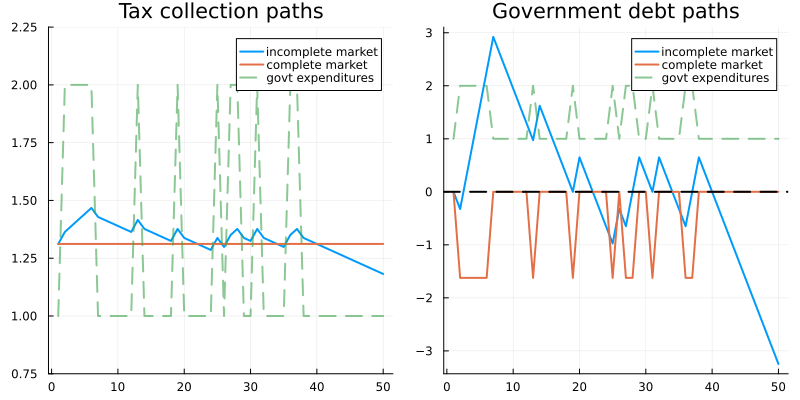
\includegraphics[width=1\textwidth]{plot.png}
                    \caption{Tax and debt policy in complete and incomplete markets. Computed using QuantEcon Julia package.} 
                \end{figure}

            \end{frame}
\end{document}